\section{Experiment}

\subsection{Experimental Setup}

\paragraph{Datasets}
To comprehensively evaluate the reasoning capabilities of RAG systems, we conduct experiments on two distinct categories of tasks: \textbf{Deep Reasoning Tasks} including HotpotQA~\citep{yang2018hotpotqa}, 2WikiMultiHopQA~\citep{2wiki} and Musique~\citep{musique} and \textbf{Broad Reasoning Tasks} including 4 subsets of UltraDomain~\citep{qian2025memorag} benchmark. 
Detailed statistics for all datasets are provided in Table~\ref{tab:dataset_stats} and Appendix.~\ref{appendix:dataset_detail}.

% \textbf{Deep Reasoning Tasks} focus on complex question answering that requires multi-step logical inference and evidence integration. We evaluate on three established multi-hop QA datasets, including HotpotQA~\citep{yang2018hotpotqa}, 2WikiMultiHopQA~\citep{2wiki} and Musique~\citep{musique}.

% \textbf{Broad Reasoning Tasks} assess the system's ability to handle domain-specific knowledge with comprehensive understanding across diverse contexts. We evaluate on four domains from the UltraDomain~\citep{qian2025memorag} benchmark.

\paragraph{Evaluation Metrics}
For \textbf{Deep Reasoning Tasks}, we follow standard QA evaluation practices with \textbf{Exact Match (EM)}(Following ToG and ToG-2~\citep{sun2023tog,ma2024tog2}, we employ a substring-based Exact Match metric.) and \textbf{F1 Score}. For \textbf{Broad Reasoning Tasks}, we adopt a multi-dimensional LLM-based evaluation approach including \textbf{Comprehensiveness}, \textbf{Diversity} and \textbf{Empowerment} following \citep{guo2024lightrag}. Metrics detail are provide Appendix.\ref{appendix:metrics}.
% \begin{itemize}
%     \item \textbf{Exact Match (EM)}: Measures the percentage of predictions that exactly match the ground truth answer.
%     \item \textbf{F1 Score}: Computes word-level overlap between predictions and ground truth answers.
% \end{itemize}

% For \textbf{Broad Reasoning Tasks}, we adopt a multi-dimensional LLM-based evaluation approach including \textbf{Comprehensiveness (Comp.)}, \textbf{Diversity (Div.)} and \textbf{Empowerment (Emp.)} due to the complexity and open-ended nature of these queries following LightRAG \citep{guo2024lightrag}.
% \begin{itemize}
%     \item \textbf{Comprehensiveness (Comp.)}: Measures how thoroughly the answer addresses all aspects of the question.
%     \item \textbf{Diversity (Div.)}: Assesses the variety of perspectives and insights provided in the answer.
%     \item \textbf{Empowerment (Emp.)}: Evaluates how well the answer enables informed understanding and judgment.
% \end{itemize}
% The LLM-based evaluation uses GPT-4o-mini as judge, with careful attention to prompt design and answer ordering to avoid positional bias. The LLM evaluation prompt is shown in Appendix.\ref{appendix:prompts}


\paragraph{Baselines}
% We compare against state-of-the-art RAG methods including GraphRAG, HippoRAG, and other established baselines from recent literature. Each baseline is evaluated under identical experimental conditions to ensure fair comparison.
We compare \model\ against the following state-of-the-art RAG methods across all datasets, including NaiveRAG~\citep{gao2023rag_survey}, ToG-2~\citep{ma2024tog2}, GraphRAG~\citep{edge2024local}, LightRAG~\citep{guo2024lightrag}, MiniRAG~\citep{fan2025minirag} and HippoRAG-2~\citep{gutiérrez2025HippoRAG2}. Baselines details can be found in Appendix.\ref{appendix:baselines}.
% All baselines are implemented using their official code repositories with consistent parameter settings to ensure fair comparison. 
For graph-based methods, we maintain identical chunk sizes (1024 tokens) and use the same LLM (Qwen2.5-32B-Instruct~\citep{qwen2.5}) for all extraction and generation tasks to eliminate model capability variations. Implementation details are provide Appendix.\ref{appendix:imple_detail}.



\subsection{Result of Deep Reasonging Benchmark}


\paragraph{Result Analysis from a Method Perspective.} Results shown in Table~\ref{tab:deep_resoning_results} represent the average of three independent reasoning experiments.
Previsou Graph-based methods like GraphRAG that rely on LLM-based graph construction show limited performance. Their performance is the lowest, particularly in terms of F1 scores as shown in Figure~\ref{fig:f1_comparison}, which can be attributed to a lack of focus on deep factual reasoning and a tendency to produce verbose responses, resulting in low token-level recall. 
More detailed precision and recall results are provided in Appendix.~\ref{appendix:pr_result}. 
ToG-2, without leveraging well-curated knowledge graphs like Freebase and Wikidata, demonstrates moderate performance in open-domain settings. 
NaiveRAG achieves competitive third-place results by avoiding graph construction limitations and relying solely on retrieved documents for response generation.
HippoRAG-2 emerges as the strongest baseline, employing an efficient embedding model with Personalized PageRank algorithm and LLM-based triple filtering to achieve second-best performance. 
However, our proposed method consistently outperforms all competitors, achieving the highest average EM (0.474) and F1 (0.345) scores across all three benchmarks. This superior performance is attributed to our novel Chunk-Triplets-Community heterogeneous graph architecture and the Multi-Agent Context Evolution and Retrieval (MACER) framework, which enables adaptive subgraph refinement and evolving query decomposition for complex reasoning tasks and overcomes the graph construction challenges that plague other graph-based RAG systems. 
Additional Baselines are provided in Appendix.\ref{appendix:add_baselines}.

\paragraph{Result Analysis from a Dataset Perspective.} As shown in Figure~\ref{fig:performance_comparison}, the average performance of the baselines and our method across the HotpotQA, 2WikiMultiHopQA, and Musique datasets generally follows a descending trend. This pattern can be attributed to the following reasons: HotpotQA~\citep{yang2018hotpotqa}: Although widely used, this dataset has been shown to provide a weaker test of multi-hop reasoning due to the presence of numerous spurious cues and shortcut signals~\citep{musique,hipporag}. Musique~\citep{musique}: A challenging multi-hop QA dataset comprising approximately requiring 2–4 hops, which emphasizes a comprehensive evaluation of multi-step reasoning abilities. Musique is designed to feature diverse and complex reasoning paths, necessitating the integration of information across multiple hops to arrive at correct answers. 

% The results demonstrate that our approach effectively addresses the limitations of existing methods by combining the structural advantages of knowledge graphs with the flexibility of document retrieval, while overcoming the graph construction challenges that plague other graph-based RAG systems. 

\begin{table*}
\centering
\caption{Exact Match (EM) and F1 scores on Deep Reasoning datasets.We highlight the \colorbox{green!80!black}{best},  \colorbox{green!40}{second-best}, and \colorbox{green!10}{third-best}methods with different background color shades.}
\small
\begin{tabular}{lcccccc|cc}
\toprule
\multirow{2}{*}{Method} & \multicolumn{2}{c}{HotpotQA} & \multicolumn{2}{c}{2WikiMultihopQA} &  \multicolumn{2}{c}{Musique} &  \multicolumn{2}{c}{Average} \\
\cmidrule(lr){2-3} \cmidrule(lr){4-5} \cmidrule(lr){6-7} \cmidrule(lr){8-9}
 & EM & F1 & EM & F1 & EM & F1 & EM & F1 \\
\midrule
NaiveRAG & \secondres{0.634} & \thirdres{0.365} & 0.382 & 0.189  & \secondres{0.230} & \thirdres{0.143} & \thirdres{0.415} & \thirdres{0.232} \\
ToG-2 & 0.308 & 0.153 & 0.401 & \thirdres{0.194}  & 0.103 & 0.105 & 0.271 & 0.151  \\
GraphRAG & 0.337 & 0.011 & \thirdres{0.439} & 0.018  & 0.109 & 0.008  & 0.295 & 0.012 \\
LightRAG  & 0.308 & 0.013  & 0.420 & 0.023 & 0.082 & 0.009  & 0.270 & 0.015  \\
MiniRAG & 0.213 & 0.012 & 0.125 & 0.018  & 0.067 & 0.007 & 0.135 & 0.012 \\
HippoRAG-2 & \thirdres{0.612} & \secondres{0.534} & \secondres{0.491} & \secondres{0.254}  & \thirdres{0.212} & \secondres{0.145} & \secondres{0.438} & \secondres{0.311} \\
\midrule
Ours  & \firstres{0.654} & \firstres{0.569} & \firstres{0.527} & \firstres{0.291} & \firstres{0.241} & \firstres{0.174} & \firstres{0.474}$_{\color{red}{\uparrow 8.2\%}}$ & \firstres{0.345}$_{\color{red}{\uparrow 10.9\%}}$ \\
\bottomrule
\end{tabular}
\label{tab:deep_resoning_results}
\end{table*}

\begin{figure*}
    \centering
    \begin{subfigure}[b]{0.49\textwidth}
        \centering
        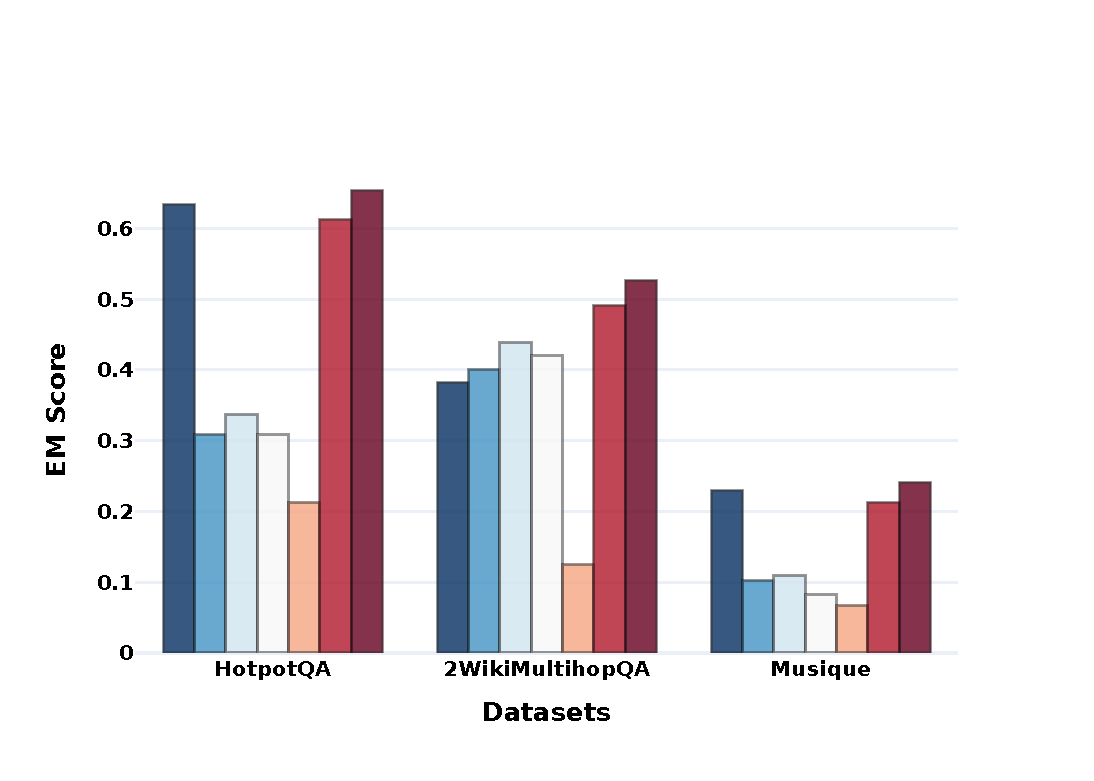
\includegraphics[width=\linewidth]{figs/em_bar_chart.pdf}
        \caption{Exact Match (EM) Score Comparison}
        \label{fig:em_comparison}
    \end{subfigure}
    \hfill
    \begin{subfigure}[b]{0.49\textwidth}
        \centering
        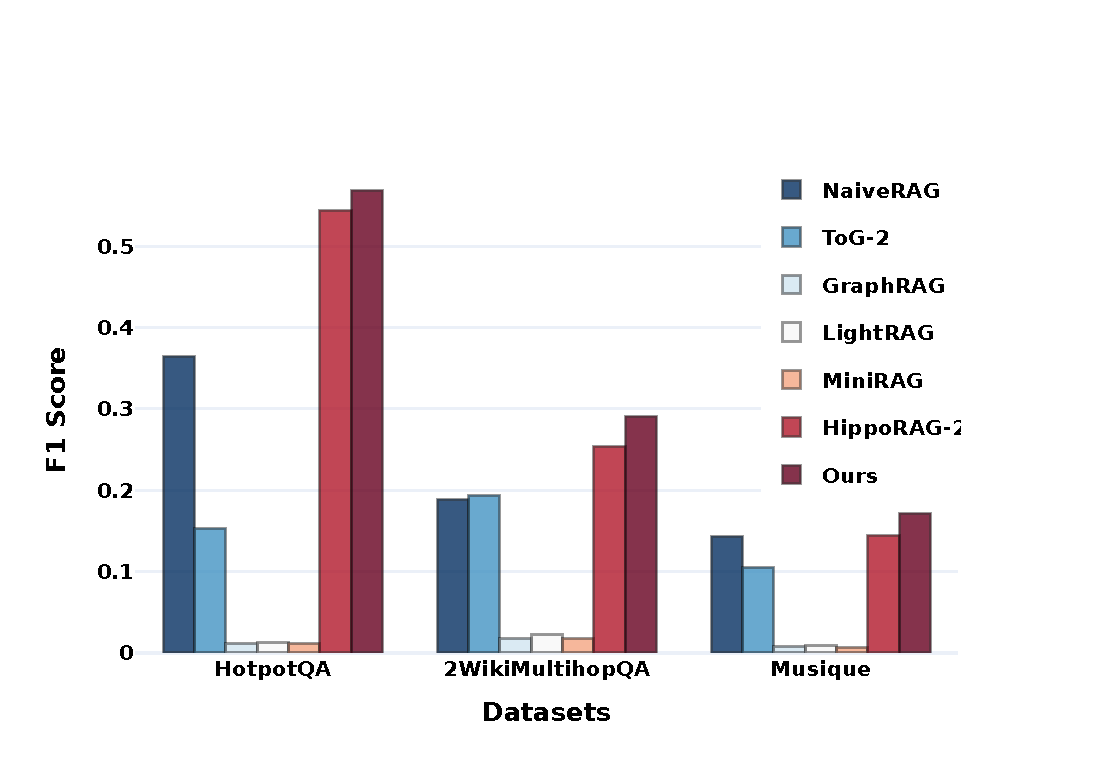
\includegraphics[width=\linewidth]{figs/f1_bar_chart.pdf}
        \caption{F1 Score Comparison}
        \label{fig:f1_comparison}
    \end{subfigure}
    \caption{Performance comparison of different RAG methods on multi-hop QA datasets. (a) Exact Match scores measure the percentage of questions where the model's answer exactly matches the ground truth. (b) F1 scores provide a harmonic mean of precision and recall for token-level answer matching. }
    \label{fig:performance_comparison}
\end{figure*}

\subsection{Result of Broad Reasoning Tasks}

\begin{figure*}
    \centering
    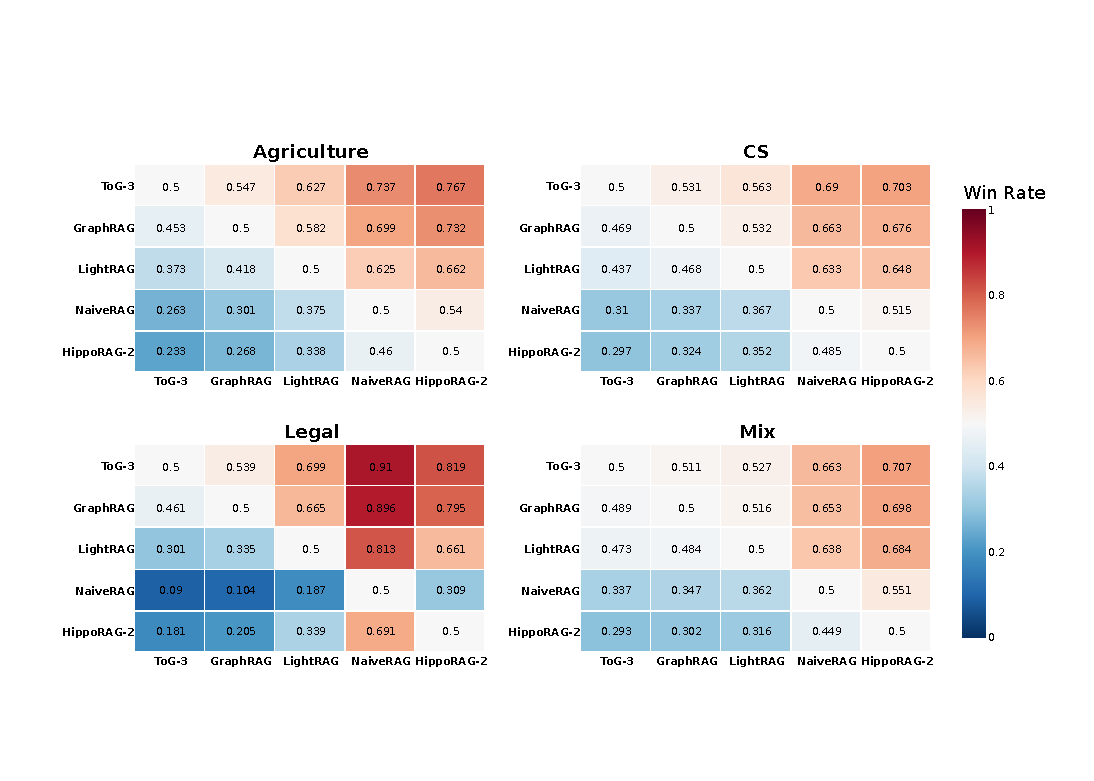
\includegraphics[width=0.95\linewidth]{figs/elo_win_rates_heatmap.pdf}
    \caption{\textbf{ELO-based Pairwise Win Rate Matrices Across Four Benchmark Datasets. }
Each heatmap visualizes win probabilities derived from direct head-to-head experimental comparisons, transformed through the ELO framework to ensure transitive consistency. The diagonal of the heatmap is set to a default value of 0.5, indicating self-comparison of the method.}
    \label{fig:elo_win_rates_heatmap}
\end{figure*}

% The comprehensive evaluation in Table~\ref{tab:braod_tasks_performance} demonstrates that ToG-3 achieves state-of-the-art performance across all benchmark datasets, with particularly significant advantages in complex reasoning tasks. 
As shwon in Figure~\ref{fig:elo_win_rates_heatmap}, The four heatmaps clearly demonstrate that the five methods can be distinctly divided into two clusters: the upper-right region (predominantly red, indicating superior performance) and the lower-left region (predominantly blue, indicating inferior performance). Specifically, ToG-3, GraphRAG, and LightRAG exhibit significantly higher win rates compared to NaiveRAG and HippoRAG-2.
Detailed win rates (\%) of baselines v.s. ToG-3 across four datasets are provided in Table~\ref{tab:braod_tasks_performance} of Appendix.~\ref{appendix:more_result_details}.
Our framework outperforms NaiveRAG by substantial margins (up 75.0\% average win rate on all four datasets), highlighting the limitations of chunk-based retrieval for complex queries. While GraphRAG shows competitive performance in comprehensiveness due to its extensive community summarization and retrival, ToG-3 achieves better balance across all metrics, particularly excelling in diversity and empowerment through its heterogeneous graph architecture that integrates chunk-level, triplet-level, and community-level information. Detailed ELO rating calculation for broad reasoning tasks can be found in Appendix.~\ref{appendix:elo_calculation}. 
% Figure.\ref{fig.case_study_regression_metrics} show a case study of CS dataset which illustrates the answer generated by ToG-3 is more comprehensive and empowering answer while GraphRAG's answer is more diverse. More case study can be found in Appendix.\ref{sec:appendix_case}. 
The multi-agent dual-evolving context retrieval mechanism enables both deep knowledge reasoning through entity-relation exploration and broad community reasoning.
% overcoming the specialization limitations of HippoRAG-2's ranked triples and Personalized PageRank algorithm (focused on deep reasoning but weak in breadth) and LightRAG's constrained contextual understanding. 
% This balanced architectural approach makes ToG-3 particularly effective for real-world applications requiring both comprehensive coverage and precise, actionable insights.
Our analysis reveals that, on average, 20\% of the samples require one evolving-context iteration, 32\% require two iterations, and 48\% require three iterations.

\begin{table*}
\centering
\caption{Ablation studies of MACER components and foundation model scaling. 
Standard ToG-3 settings incorporates all MACER components, employs the Qwen2.5-32B-instruct as the backbone LLM, and utilizes the Jina-v3-embedding model for representation encoding and Jina-reranker-v2 for reranking the retrieved evidence.
% The upper section shows that evolving query decomposition contributes most significantly to performance, while the lower section demonstrates that larger LLMs provide substantial gains over embedding model scaling.
}
\small
\begin{tabular}{lcccccc|cc}
\toprule
\multirow{2}{*}{Ablation Setting} & \multicolumn{2}{c}{HotpotQA} & \multicolumn{2}{c}{2WikiMultihopQA}  & \multicolumn{2}{c}{Musique} & \multicolumn{2}{c}{Average} \\
\cmidrule(lr){2-3} \cmidrule(lr){4-5} \cmidrule(lr){6-7} \cmidrule(lr){8-9}
& EM & F1 & EM & F1 & EM & F1 & EM & F1 \\
\midrule
% Standard ToG-3 settings & 0.654 & 0.569 & 0.527 & 0.291 & 0.241 & 0.174 & 0.474 & 0.345 \\
% \midrule
\rowcolor{gray!30}
\multicolumn{9}{l}{\textbf{MACER Components Ablation}} \\
w/o Evolving Query & 0.614 & 0.495 & 0.440 & 0.227 & 0.198 & 0.141 & 0.417 & 0.288 \\
w/o Evolving Sub-Graph & 0.629 & 0.525 & 0.486 & 0.258 & 0.223 & 0.158 & 0.446 & 0.314 \\
w/o Community Node & 0.656 & 0.572 & 0.514 & 0.283 & 0.236 & 0.169 & 0.469 & 0.341 \\
\midrule
\rowcolor{gray!30}
\multicolumn{9}{l}{\textbf{Foundation Model Scaling Abalation}} \\
\rowcolor{gray!10}
\multicolumn{9}{l}{\textbf{LLM Model}} \\
Qwen2.5-14B & 0.587 & 0.521 & 0.480 & 0.255 & 0.218 & 0.154 & 0.428 & 0.310 \\
Qwen2.5-72B & 0.683 & 0.592 & 0.550 & 0.305 & 0.255 & 0.182 & 0.496 & 0.360 \\
\rowcolor{gray!10}
\multicolumn{9}{l}{\textbf{Embedding Model}} \\
Qwen3-Embed-0.6B & 0.653 & 0.571 & 0.532 & 0.294 & 0.244 & 0.176 & 0.476 & 0.347 \\
Qwen3-Embed-4B & 0.658 & 0.577 & 0.535 & 0.296 & 0.247 & 0.179 & 0.480 & 0.351 \\
\bottomrule
\end{tabular}
\label{tab:ablation_studies}
\end{table*}

Detailed comparison of time and token Consumption across different methods are provided in Appendix.\ref{appendix:computation_cost}.
Case studies of ToG-3 retrieval and response output are provided in Appendix.~\ref{appendix:case_study}.



\subsection{Abalation Study}

\paragraph{Abalation Study of MACER component}

Our ablation study reveals the relative importance of each MACER component for deep reasoning performance. The most significant performance degradation occurs when removing the evolving query mechanism (average performance drop of 12.0\% in EM and 16.5\% in F1), underscoring its critical role in complex question answering, expecially when using smaller LLMs. 
% The iterative query decomposition enables the framework to break down multifaceted questions into tractable sub-problems, which is essential for navigating the heterogeneous graph structure. 
Removing subgraph refinement causes a moderate performance decrease (average drop of 6.0\% in EM and 9.0\% in F1), indicating its importance in adapting the knowledge structure to the specific reasoning context. Interestingly, community nodes show the smallest impact on deep reasoning tasks (a slight drop in the average EM and F1 scores), suggesting that while they contribute to performance, the chunk and triplet representations carry most of the relevant information for precise answer generation. 
However, in broad reasoning tasks, community nodes are essential for comprehensive coverage and diversity, highlighting the complementary roles of different node types in our heterogeneous graph architecture.
Note that the reranker agent also delivers a 4.6\% improvement in EM and a 10.6\% improvement in F1. This is because, during multi-turn RAG processes, an excessive amount of retrieved evidence can otherwise impair the response quality of the responser agent.


\paragraph{Abalation Study of used foundation model}

The foundation model scaling analysis reveals several important patterns. First, LLM capacity has a substantially greater impact on performance than embedding model size. Scaling from Qwen2.5-14B to Qwen2.5-72B yields a 15.9\% average improvement in EM scores, highlighting the critical role of reasoning capability in complex QA tasks. Second, larger embedding models provide consistent but more modest improvements. Qwen3-Embed-0.6B shows a slight average EM improvement over jina-embeddings-v3, while Qwen3-Embed-4B provides a 1.7\% improvement. This suggests that while retrieval quality matters and larger embedding models contribute to better performance, the LLM's reasoning capacity remains the primary bottleneck for complex reasoning tasks. These findings provide practical guidance for resource allocation in real-world deployments.
% emphasizing that investing in larger LLMs yields greater returns than investing in larger embedding models.



